\section{Express.js}

\textbf{Express} ist die wohl bekannteste Library zum Erstellen von Server-Software mit \textit{Node.js}.~\cite{serby2012} Dabei hat sie das Ziel durch ihre minimalistische und flexible Art eine schnelle und robuste Grundlage für Serverprojekte jeglicher Art in Node.js zu bieten. Mit Express ist es möglich, einfache APIs zu schreiben, aber auch komplexe Web-Projekte umzusetzen.

\subsection{Das Express \glqq Hello world!\grqq}

Die wohl einfachste Express-Anwendung gibt bei Aufruf der Root-Route einfach ein \glqq Hello world!\grqq\space zurück.

\begin{code}[htp]
    \begin{center}
        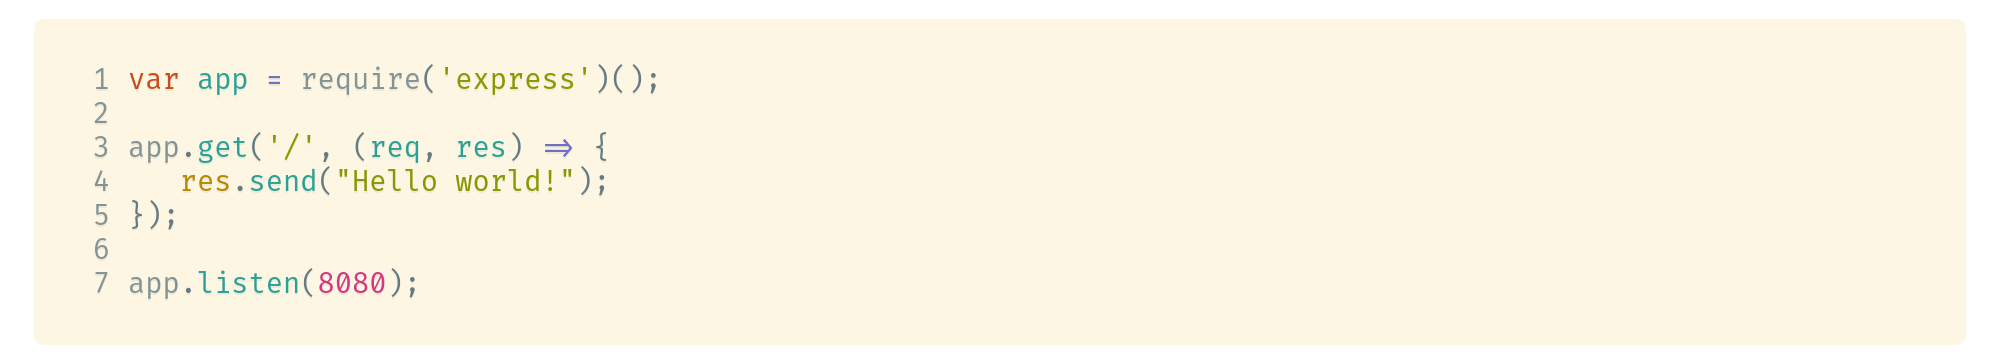
\includegraphics[width=1\textwidth]{images/Dependencies/express.png}
        \vspace{-25pt}
        \caption{\glqq Hello world!\grqq\space mit Express.js}
    \end{center}
\end{code}

\begin{figure}[ht]
    \centering
    
\includegraphics[width=0.8\textwidth]{images/Dependencies/helloworld.png}
    \caption{Die Ausgabe einer \glqq Hello world!\grqq -Seite mit Express.js}
\end{figure}

Natürlich ist die Anwendung von Express in Sokka wesentlich komplexer, allerdings sieht man in diesem Beispiel schon sehr gut die grundlegende Funktionsweise der Library .

\subsection{Rolle von Express in Sokka}

Das \nameref{backend} von Sokka stützt sich komplett auf die Funktion von Express. Jede API-Route des Servers wird durch Express erstellt und jede Anfrage an den Server wird von Express unterhalten.